% Created with jtex v.1.0.20
\documentclass{article}
\usepackage{arxiv}

\usepackage[utf8]{inputenc} % allow utf-8 input
\usepackage[T1]{fontenc}    % use 8-bit T1 fonts
\usepackage{hyperref}       % hyperlinks
\usepackage{url}            % simple URL typesetting
\usepackage{datetime}       % show dates in the title block
\usepackage{booktabs}       % professional-quality tables
\usepackage{amsfonts}       % blackboard math symbols
\usepackage{nicefrac}       % compact symbols for 1/2, etc.
\usepackage{microtype}      % microtypography
\usepackage{graphicx}
\usepackage{natbib}
\usepackage{doi}
\usepackage{xcolor}
\usepackage{listings}

%%%%%%%%%%%%%%%%%%%%%%%%%%%%%%%%%%%%%%%%%%%%%%%%%%
%%%%%%%%%%%%%%%%%%%%  imports  %%%%%%%%%%%%%%%%%%%
\usepackage{amsmath}
\usepackage{framed}
%%%%%%%%%%%%%%%%%%%%%%%%%%%%%%%%%%%%%%%%%%%%%%%%%%


\hypersetup{colorlinks = true,
linkcolor = purple,
urlcolor  = blue,
citecolor = cyan,
anchorcolor = black}

\title{Homework 1}

\newdate{articleDate}{20}{1}{2025}
\date{\displaydate{articleDate}}

\makeatletter
\let\@fnsymbol\@arabic
\makeatother

\author{Jacob Cunningham\footnotemark[1]\\
}

% Uncomment to override  the `A preprint' in the header
\renewcommand{\headeright}{ME 2060}
\renewcommand{\undertitle}{ME 2060: Numerical Methods}
\renewcommand{\shorttitle}{}

%% Add PDF metadata to help others organize their library
%% Once the PDF is generated, you can check the metadata with
%% $ pdfinfo template.pdf
\hypersetup{
pdftitle={\@title},
pdfsubject={},
pdfauthor={\@author},
pdfkeywords={Numerical Methods,Mechanical Engineering},
addtopdfcreator={Written in Curvenote}
}

\begin{document}
\maketitle
\footnotetext[1]{Correspondence to: jjc132@pitt.edu}

\begin{abstract}
Homework discussion, calculations, and answers are provided herein.
\end{abstract}

\keywords{Numerical Methods, Mechanical Engineering}

\section{Effects of roundoff and truncation errors on numerical accuracy}

The one-sided finite difference scheme to approximate the first derivative of a function $f$ is defined as:

\begin{equation}
\label{equ-osfd}
f_{h}(x) = \frac{f(x + h) - f(x)}{h} \approx f'(x),
\end{equation}

where $h$ is the step size if no roundoff error exists, then the accuracy of the scheme is dermined soley by \textbf{truncation error}

\begin{equation}
\label{equ-truncation-error}
t_{e}(h) = | f'(x) - f_{h}(x) | = \mathscr{O}(h),
  \quad
  f'(x) = f_{h}(x) + \mathscr{O}(h),
\end{equation}

where the big $\mathscr{O}$ - notation means there exists a constant $K$ such that $\mathscr{O} < K \cdot h$ for all $h$. In the presence of roundoff errors, $x$ cannot be represented exactly; instead, it is represented by the rounded value $\tilde{x}$ with the associated roundoff error $r = |\tilde{x} - x |$.

\subsection{Part A}

Show that the total error of the finite-difference approximation consists of both truncation error $t_{e}(h)$ due to the finite-difference scheme and the roundoff error $r$:

\begin{equation}
\label{equ-fd-error}
\epsilon (h) := |f'(x) - f_{h}(\tilde{x})| = \mathscr{O}(h) + \frac{r}{h}
\end{equation}

\textbf{Hint}: Start from $f'(x) = f_{h}(x) + \mathscr{O}(h)$, and consider that the computation of the finite difference $f_{h}(x)$ approximation already involves roundoff errors, e.g., $f(x) = \tilde{f}(x) + r$, $f(x + h) = \tilde{f}(x) + h + r$.


\bigskip
\centerline{\rule{13cm}{0.4pt}}
\bigskip

When accounting for rounding error, the computed version of (\ref{equ-osfd}) is:

\begin{equation}
\label{equ-1A-calc-1}
\tilde{f}_{h}(x) = \frac{\tilde{f}(x + h) - \tilde{f}(x)}{h},
\end{equation}

where $\tilde{f}(x + h)$ and $\tilde{f}(x)$ are the computed values of $f(x + h)$ and $f(x)$, respectively. Since the computed values are equal to the exact values plus rounding error, (\ref{equ-1A-calc-1}) can be reduced:

\begin{align*}
  \tilde{f}_{h}(x) &= \frac{(f(x + h) + r_1) - (f(x) + r_2)}{h} \\
  &= \frac{f(x + h) - f(x) + (r_1 - r_2)}{h} \\
  &= \frac{f(x + h) - f(x)}{h} + \frac{r_1 - r_2}{h} \\
  &= f_{h}(x) + \frac{r_1 - r_2}{h}
\end{align*}

This can be rewritten as:

\begin{equation}
\label{equ-1A-calc-2}
\tilde{f}_h(x) = f_{h}(x) + \frac{r}{h},
\end{equation}

where $r = r_1 - r_2$.

The important step here is to realize that the rounding errors at $\tilde{f}(x + h)$ and $\tilde{f}(x)$ are not necessarily the same value. Substituting (\ref{equ-1A-calc-2}) into (\ref{equ-truncation-error}) gives:

\begin{align*}
  f'(x) &= (\tilde{f}_{h}(x) - \frac{r}{h}) + \mathscr{O}(h) \\
  &= \tilde{f}_{h}(x) - \frac{r}{h} + \mathscr{O}(h)
\end{align*}

Since rounding error would add error contribution the result can be rewritten as:

\begin{equation}
\label{equ-1A-calc-3}
f'(x) = \tilde{f}_{h}(x) + \frac{r}{h} + \mathscr{O}(h)
\end{equation}

The difference between the exact derivative and the computed derivative using this scheme is thus:

\begin{equation*}
f'(x) - \tilde{f}_{h}(x) = \mathscr{O}(h) + \frac{r}{h}
\end{equation*}

Since both error contributions are always positive:

\begin{equation}
\label{equ-1A-calc-4}
|f'(x) - \tilde{f}_{h}(x) | = \mathscr{O}(h) + \frac{r}{h},
\end{equation}

which is equivalent to (\ref{equ-fd-error}).

\begin{framed}
\textbf{Answer 1A}\\
The deriviation above shows how (\ref{equ-osfd}) can be written as (\ref{equ-1A-calc-1}) when accounting for rounding error. (\ref{equ-1A-calc-1}) was reduced to (\ref{equ-1A-calc-2}) and substituted into (\ref{equ-truncation-error}) to give (\ref{equ-1A-calc-3}) which was rearranged to (\ref{equ-1A-calc-4}) and is equivalent to (\ref{equ-fd-error}).
\end{framed}

\subsection{Part B}

From Part A, what can you say about the numerical accuracy of the finite difference scheme as the step size $h$ is continually decreased?


\bigskip
\centerline{\rule{13cm}{0.4pt}}
\bigskip

\begin{framed}
\textbf{Answer 1B}\\
The roundoff error term $r/h$ will dominate and roundoff errors will be amplified. Conversely if $h$ is increased the truncation error term will dominante. This implies that there is probably an optimal step size to balance both error terms.
\end{framed}

\subsection{Part C}

The second order central difference approximation is defined as

\begin{equation}
f_{h}^{c}(x) = \frac{f(x + h) - f(x - h)}{2h} \approx f'(x)
\end{equation}

and has a truncation error of $t_{e}(h) = |f'(x) - f_{h}^{c}(x) | = \mathscr{O}(h^2)$.

Within the notebook \texttt{Week2\_FD\_students.ipynb} available on Canvas Module 1, add a function to evaluate the finite difference approximation $f_{h}^{c}$ for the derivative of $f(x) = \sin (x)$ with step size $h$ at a fixed $x = x_0 = 1$. For the same array $h$ of step sizes as in the notebook, calculate the array consisting of errors between the finite difference approximation $f_{h}^{c}$ and the exact dervative $f'$. Plot the approximation error for the central differences scheme as a function of step size $h$. Display your plot in log format in addition to the previous plot for forward differences.


\bigskip
\centerline{\rule{13cm}{0.4pt}}
\bigskip

\begin{figure}[h]
\centering
\begin{lstlisting}[language=Julia, caption={Numerical Error Calculation in Julia}]
# Packages used
import Plots as plt
import LaTeXStrings as ltx

# One -sided finite difference approximation
function fh(x::Real, h::Vector{<:Real}, f::Function)
    return (f.(x .+ h) . - f.(x)) ./ h
end

# Second order central difference approximation
function fch(x::Real, h::Vector{<:Real}, f::Function)
    return (f.(x .+ h) . - f.(x . - h)) ./ (2 * h)
end

# Total error (note rounding error implicitly included)
function eps(f_exact::Real, f_num::Vector{<:Real})
        return abs.(f_exact . - f_num)
end

# Fixed x and same h array
x = 1.0
n = 1:15
h = 10.0 .^ -n

# Numerical derivatives
fh_sin = fh(x, h, sin)
fch_sin = fch(x, h, sin)

# Exact derivative
f_deriv_sin = cos(x)

# Total errors
eps_fh_sin = eps(f_deriv_sin, fh_sin)
eps_fhc_sin = eps(f_deriv_sin, fch_sin)

# Plots
plt.plot(h, eps_fh_sin,
    yaxis=:log10, xaxis=:log10,
    label="Forward Difference",
    lc=:black, lw=2, ls=:solid)

plt.plot!(h, eps_fhc_sin,
    label="Central Difference",
    lc=:black, lw=2, ls=:dash)

plt.plot!(legend=:bottomleft)
plt.title!(ltx.L"Numerical Error $\epsilon (h)$ vs. Step Size $h$")
plt.xlabel!(ltx.L"\log h")
plt.ylabel!(ltx.L"\log\epsilon (h)")
plt.annotate!(1e -13, 1e -9, ltx.L"$f(x) = \sin(x)$")
\end{lstlisting}
\caption[]{Plotting approximation error for central differences schemen and forward difference scheme.}
\label{code-p1C}
\end{figure}

\begin{verbatim}
# Packages used
import Plots as plt
import LaTeXStrings as ltx

# One -sided finite difference approximation
function fh(x::Real, h::Vector{<:Real}, f::Function)
    return (f.(x .+ h) . - f.(x)) ./ h
end

# Second order central difference approximation
function fch(x::Real, h::Vector{<:Real}, f::Function)
    return (f.(x .+ h) . - f.(x . - h)) ./ (2 * h)
end

# Total error (note rounding error implicitly included)
function eps(f_exact::Real, f_num::Vector{<:Real})
        return abs.(f_exact . - f_num)
end

# Fixed x and same h array
x = 1.0
n = 1:15
h = 10.0 .^ -n

# Numerical derivatives
fh_sin = fh(x, h, sin)
fch_sin = fch(x, h, sin)

# Exact derivative
f_deriv_sin = cos(x)

# Total errors
eps_fh_sin = eps(f_deriv_sin, fh_sin)
eps_fhc_sin = eps(f_deriv_sin, fch_sin)

# Plots
plt.plot(h, eps_fh_sin,
    yaxis=:log10, xaxis=:log10,
    label="Forward Difference",
    lc=:black, lw=2, ls=:solid)

plt.plot!(h, eps_fhc_sin,
    label="Central Difference",
    lc=:black, lw=2, ls=:dash)

plt.plot!(legend=:bottomleft)
plt.title!(ltx.L"Numerical Error $\epsilon (h)$ vs. Step Size $h$")
plt.xlabel!(ltx.L"$\log h$")
plt.ylabel!(ltx.L"$\log\epsilon (h)$")
plt.annotate!(1e -13, 1e -9, ltx.L"$f(x) = \sin(x)$")
\end{verbatim}

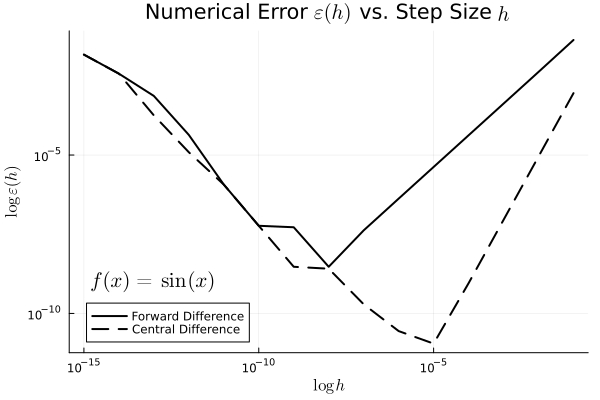
\includegraphics[width=0.7\linewidth]{files/1c7bae06802b8646ae520dfa46d49f2d.png}

\begin{framed}
\textbf{Answer 1C}\\
The figure above shows that the central difference scheme is superior to the forward difference scheme.
\end{framed}

\subsection{Part D}

Now repeat the same above steps for the function $g(x) = \sin (100x)$ and its derivative $g'(x)$. Add your plots for the forward difference and central difference numerical errors to the same plot. Make sure to use a different linestyle, and specify your legend entries. Looking at your plot, what can you say about the accuracy of each method to approximate the derivative for $\sin (x)$ and $\sin (100x)$ at $x_{0} = 1$? Can you explain why?

\begin{framed}
\textbf{Answer 1D}\\
Answer goes here.
\end{framed}

\section{Errors in Scientific Computing}

The sine function is given by the infinite series

\begin{equation}
\sin x = x - \frac{x^3}{3!} + \frac{x^5}{5!} -\frac{x^7}{7!} + \cdots
\end{equation}

\subsection{Part A}

Calculate the forward and backward errors if we approximate the sine function by using only the first term in the series for $x = 0.1, \; 0.5, \; 1.0$.

\begin{framed}
\textbf{Answer 2A}\\
Answer goes here.
\end{framed}

\subsection{Part B}

Calculate the forward and backward errors if we approximate the sine function by using only the first two terms in the series for $x = 0.1, \; 0.5, \; 1.0$.

\begin{framed}
\textbf{Answer 2B}\\
Answer goes here.
\end{framed}

\section{Condition Number \& Stability}

This is Exercise 1 from Section 1.4, page 26 of \cite{driscoll}. Exercises are also available at the end of each section of a chapter in the online textbook. Refer to your textbook for cross-referenced equations and tables.

Consider the formulas

\begin{equation}
f(x) = \frac{1 - \cos x}{\sin x},
  \quad
  g(x) = \frac{2 \sin^2 x/2}{\sin x},
\end{equation}

which are mathematically equivalent, but they suggest evaluation alrogirthms that can behave quite differently in floating point arithmetic.

\subsection{Part A}

Using (1.2.6), find the relative condition number of $f$. Note that because $f$ \& $g$ are mathematically equivalent, their condition numbers are the same. Show that the condition number approaches to 1 as $x \to 0$, which means it is possible to compute the function accurately near zero.

\begin{framed}
\textbf{Answer 3A}\\
Answer goes here.
\end{framed}

\subsection{Part B}

Compute $f(10^{ -6})$ using a sequence of four elementary operations. Using Table 1.1 on page 13, make a table like the one shown in Demo 1.4.1 in the book that shows the result of each elementary result and the numerical value of the condition number of that step.

\begin{framed}
\textbf{Answer 3B}\\
Answer goes here.
\end{framed}

\subsection{Part C}

Repeat Part B for $g(10^{ -6})$, which has six elementary steps.

\begin{framed}
\textbf{Answer 3C}\\
Answer goes here.
\end{framed}

\subsection{Part D}

Based on your answers to Part B \& C, is $f(10^{ -6})$ or $g(10^{ -6})$ more accurate (provide your answer as Markdown text in your Jupyter notebook)?

\begin{framed}
\textbf{Answer 3D}\\
Answer goes here.
\end{framed}

\section{Floating Point Arithmetic}

Create an example calculation to demonstrate that floating point addition is not associative. Repeat the exercise for floating point multiplication.

\begin{framed}
\textbf{Answer 4}\\
Answer goes here.
\end{framed}


\section*{Original article}
\footnotesize
This article is available online at the following URL: \href{https://jacob-cunningham-ds.github.io/me2060/hw1-code-cunningham}{https://jacob-cunningham-ds.github.io/me2060/hw1-code-cunningham}
\normalsize

\bibliographystyle{unsrtnat}
\bibliography{main.bib}

\end{document}
